\section{Introduction}
\label{sec:introduction}
%
This is the \ac{GIPER} instrument proposal in answer to the \ac{ESA} \ac{AO}\cite{JUICE_AO} for the \ac{JUICE} mission. An \ac{IPR} is part of the Model Payload suggested by the  JUICE Science Study Team\cite{yellowbook}. This document will show that the \ac{GIPER} instrument will be able to provide high profile scientific investigations that are in accordance with the scientific and technical requirements of the \ac{JUICE} mission.
%
\subsection{JUICE Mission Overview}
The \ac{JUICE} mission is an \ac{ESA} L1 class science mission selected in May 2012 as part of the \ac{ESA} "Cosmic Vision" programme. The \ac{JUICE} mission originated from a reformulation of the EJSM-Laplace mission into a European-led mission. The mission is scheduled for launch in 2022 and arrival at Jupiter in 2030 where it will be inserted into a Jupiter orbit. It will include numerous flybys of Callisto, two Europa flybys, insertion into circular Ganymede orbits of three different altitudes and eventually de-orbit onto the Ganymede surface. 
%
%
%
 
\section{Scientific Objectives}
%scientific investigation. Overall instrument capability, global mission goal, anticipated scientific performance on instrument, compared to similar instruments, discussion of synergies between different observations, list of assuptions for achieving science objectives: SC performance, orbit, other payloads, ground segment.
%
The scientific outcome of this instrument proposal is in accordance with ESA \ac{SciRD}\cite{SciRD} and addresses many of the scientific investigations proposed in the ESA JUICE Assessment Study Report\cite{yellowbook}.
%
%

\subsection{Introduction \label{sub:Introduction-science}}

Ganymede is the largest moon in the Jovian System and one of the four
Galilean moon. It was discovered in 1610 by Galileo Galilei. With
a mean radius of 2634~km Ganymede is the largest moon in the Solar
System and even larger than the planet Mercury. It travels around
Jupiter in an orbit with a semi-major axis of $1070400$~km and an
eccentricity of 0.00013. It is therefore the third of the Galilean
moons. 

It is believed that Ganymede consists mainly of 3 layers which are
fully differentiated. The core consists of a hot iron alloy which
is responsible for generating the intrinsic magnetic field. The second
layer is made of heavier rocky material and the third layer consists
mainly of water ice. The icy surface is expected to be around 800~km
thick. On the boundary between the icy and the rocky layer large oceans
of liquid water may be present.


\subsubsection{The surface composition of Ganymede}

The main understanding of the surface composition and the underlying
processes of forming Ganymede originates from the Galileo mission
from 1989 to 2003. The objective of the Galileo mission was to investigate
the Jupiter system. Therefore most instruments were focusing on imaging,
measuring particles and fields and no subsurface measuring instrument
was available. An image of the Ganymede surface taken from the Galileo
orbiter is show in figure \ref{fig:Ganymed-true-color}. It consists
mainly of water ice and is basically separated into regions with a
low albedo, often referred to as dark terrain, which covers about
35~\% of the surface and regions of high albedo, named bright terrain
respectively, which covers 65~\%. The boundaries between dark and
bright terrain are sharp and distinct. The dark terrain is covered
with a much higher amount of impact craters. It is therefore believed
to be much older than the bright terrain%
\begin{comment}
dates missing
\end{comment}
. Stereo images suggests that the dark furrow terrain is generally
higher than the grooved bright terrain. This leads to the idea that
bright terrain has probably formed by tectonic processes of the (former)
dark terrain together with transport processes of snow or water to
the surface like cryo-volcanism (see also section \ref{sub:volcanism})
thereby smoothing the surface. Impact craters of meteoroids therefore
show up as bright white spots on the white terrain. 

\begin{figure}
\begin{centering}
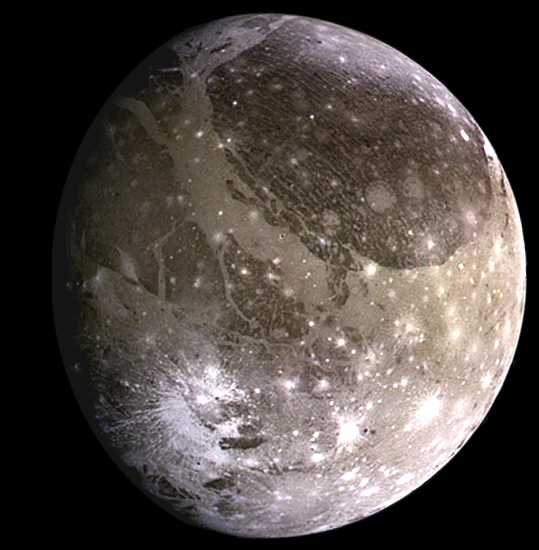
\includegraphics[width=0.70\textwidth]{Figures/Ganymede_true_color}
\par\end{centering}

\caption{\label{fig:Ganymed-true-color}}


\end{figure}



\subsubsection{Formation of the surface and sub-surface processes\label{sub:volcanism}}

The processes causing the formation of the bright terrain from the
ancient dark terrain are believed to be tectonics and cryo-volcanism
although they are still not fully understood and part of active discussions%
\begin{comment}
ref
\end{comment}
. Most models need a heat source strong enough to (partly) melt sub-surface
layers. The current orbital parameters of Ganymede would not be sufficient
to produce enough heat by tidal forces, orbital calculations suggest
that Ganymede had a period where the eccentricity of its orbit reached
as high as 0.03 %
\begin{comment}
ref
\end{comment}
{} which would cause enough tidal heating to melt parts of the icy interior. 

Another unknown problem is the transport of the then (partly) molten
ice or slush to the surface in order to fill graben. One proposition
is that icy ,,volcanoes`` ejected low-viscous liquid water which
then flooded the graben before freezing. So far no strong evidences
for this volcanism like downstream patterns on the horsts or ejection
centers. This may be because the resolution of the images obtained
by the Galileo and Voyager missions do not have a high enough resolution,
the areas for which high resolution pictures are available do not
have pronounced enough evidences or there are just not existent%
\begin{comment}
ref
\end{comment}
. Another problem is that water or slush have a higher density than
ice thus if tidal heating would melt ice the water or slush would
sink deeper instead of rising to the top.

An approach to solve this issue which would also explain why there
is no ice on top on the horsts and the lack of flooding tracks is
that tectonics resurfaced the dark terrain to contain horsts and grabens.
These apply different pressure to the underlying terrain. These pressure
gradients could actually lead to the circumstance that material with
a negative buoyancy like water or slush could move upwards but only
below the grabens. When the graben are filled with ice, the process
automatically stops because the necessary pressure imbalance from
the terrain disappears hence no ice could reach the high horsts%
\begin{comment}
ref
\end{comment}
. 

In figure \ref{fig:gradients} an example calculation for the gradients
due to terrain imbalance is presented. The terrain was modeled as
a sine wave with 30~km wavelength and an amplitude of 1~km (2~km
peak-to-peak) as shown in the top graphic of figure \ref{fig:gradients}.
\begin{figure}
\begin{centering}
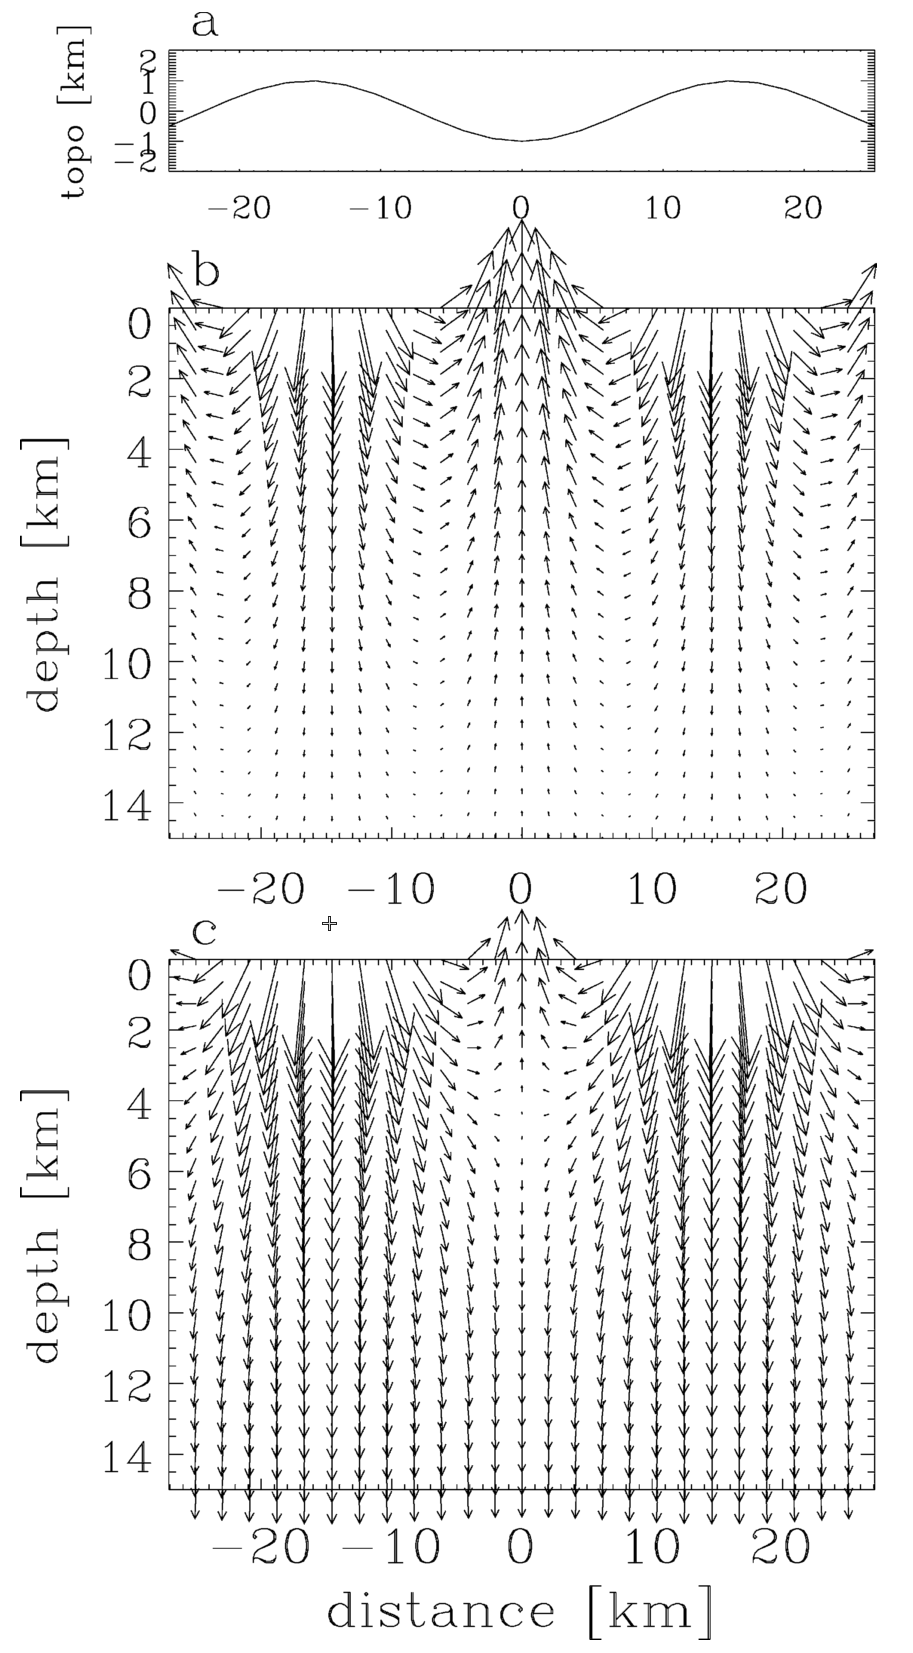
\includegraphics[width=0.70\textwidth]{Figures/gradients}
\par\end{centering}

\caption{\label{fig:gradients}}


\end{figure}
 The vector plot in the middle shows the resulting pressure gradients.
As can be seen underneath the graben they are directed upwards but
decrease exponentially with depth. The lower vector plot shows the
resulting gradients when considering water with a negative buoyancy.
As can be seen water could only move up to the surface when it is
created in a depth below 5~km. Further calculations performed by
Showman, Mosqueira et al. estimate that depth from where water or
slush can rise to the surface ranges from 5~km to 10~km. A possible
problem with this model may be that is would need at lease 1 million
years to transport enough water to the surface in order to fill grabens,
but the graben could relax gravitationally earlier and thus stop the
upward flow. 

In order to find the dominant processes for the resurfacing of Ganymede's
dark terrain it would be essential to acquire measurements from the
subsurface interior additionally to (new) surface pictures. Ganymede
can be seen as a prototype for an icy body. Therefore investigating
the tectonic processes of Ganymede and its surface evolution will
not only provide more information about the formation of Ganymede
but also of its siblings Europa and Callisto as well as icy bodies
in general %
\begin{comment}
ref 
\end{comment}
.


\subsection{Scientific Goals\label{sub:Scientific-Goals}}

Based on the short scientific introduction of Ganymede from section
\ref{sub:Introduction-science} the following scientific goals can
be identified:
\begin{itemize}
\item Map the interior below the surface of Ganymede to get more insight
about different layers and their composition. 
\item Find evidences for the tectonic processes which created the horsts
and grabens of the grooved terrain
\item Find evidences for or against different cryo-volcanism scenarios
\item Get a more detailed map of the surface terrain compared to stereoscopic
imaging
\item Possibility to find habitable zones 
\item yada yada yada
\end{itemize}

\subsection{Scientific Performance Requirements}

In order to achieve the goals described in section \ref{sub:Scientific-Goals}
the instrument should be able to penetrate the surface to at least
5~km. Attenuation of radar waves in the lower MHz spectrum in ice
is quite small which is beneficial for a high penetration depth, but
although it is quite certain that the upper surface mainly consists
of water ice there might be significant amounts of rocky material
at some parts due to the many meteoroid impacts after the accretion
phase of Ganymede. Therefore an appropriate margin for the penetration
depths should be considered. 

The vertical resolution should be in the range of 10~m -- 35~m to
give the chance to resolve the position and offset of the identified
layers with high accuracy. A typical width for the groves of the terrain
is 10~km, thus the horizontal resolution should not exceed this value
in order to correlate different vertical layers to the surface terrain. 

As the goal is to create a map of the whole surface of Ganymede it
is expected that even after preprocessing and compression a large
amount of data will be collected. An appropriate downlink capacity
should be reserved for the mission.
%
%
\section{Instrument Design}
\label{IPR_design}
The technical design of this \ac{IPR} proposal is in accordance with ESA Model Payload Definition Document for the Jupiter Icy Moons Explorer \cite{JGO_Payload_def} and addresses the instrument concept, design and its characteristics 
\subsection{Instrument Concept}
\ac{IPR} is an active radar sounding instrument which is based on the transmission of the electromagnetic waves at low frequency and uses reflected echoes from the surface and subsurface to image the subsurface structure that contains the information about the interfaces of different subsurface layers. Thanks to the relatively low frequency and the nadir-looking geometry, only a portion of the transmitted pulse is backscattered from the surface, while a significant part of the pulse is propagated to the subsurface icy layers \cite{Gany_SRS}. The coherent echoes backscattered from the subsurface interfaces within each resolution cell (defined by the along-track and across-track resolutions) are detected by the receiver and visualized in the resulting radargram \cite{Gany_SRS}. Working principle of the \ac{IPR} for \ac{JGO} is shown in figure \ref{fig:IPR_concept}. Off-nadir echo (e.g from point B in figure \ref{fig:IPR_concept}) will reach the antenna at the same time as the subsurface echo thus masking it. 
So clutter estimation and rejection is done in signal processing for both along track and across track direction.\\
%
\begin{figure}[bht]
\centering
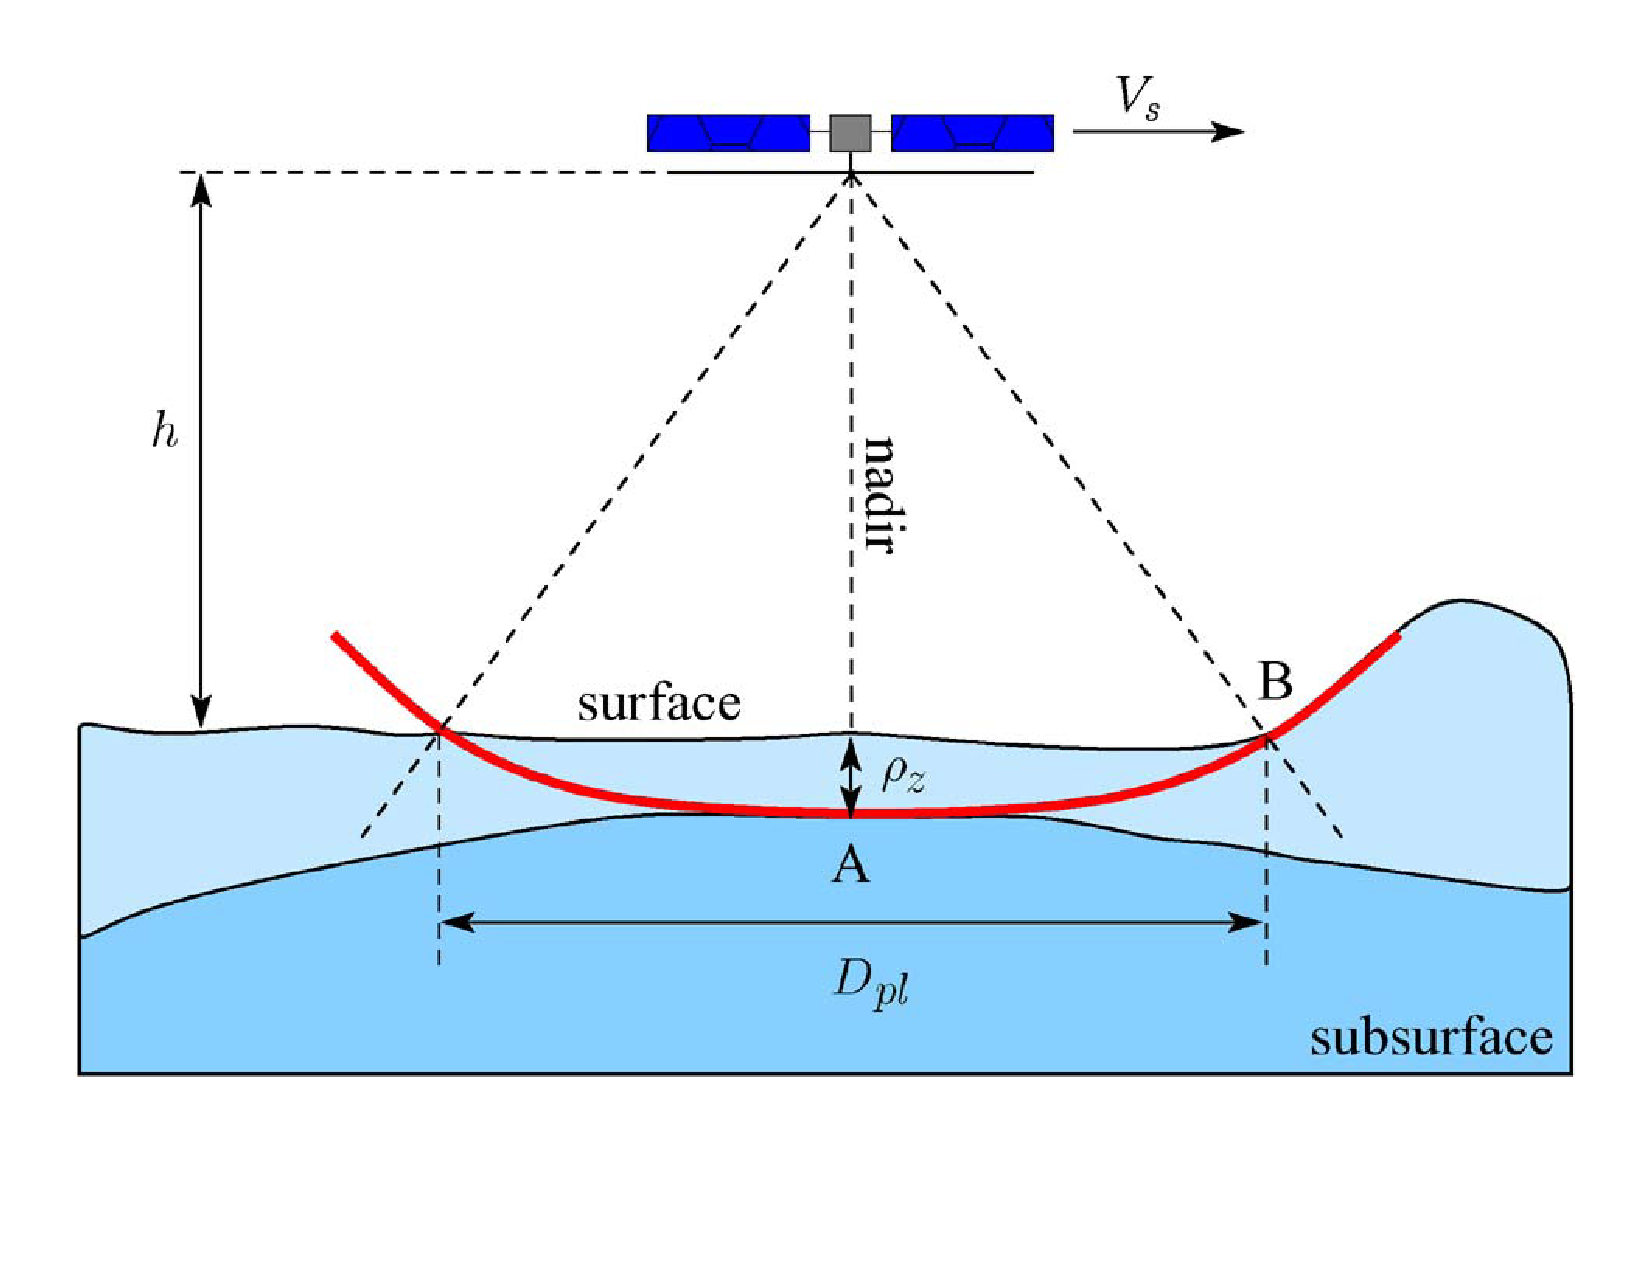
\includegraphics[scale=0.5]{Figures/IPR_Concept.pdf}
\caption{Geometry of \ac{IPR} sounder instrument \cite{Gany_SRS}} 
\label{fig:IPR_concept}
\end{figure}
%
\subsection{Instrument Description}
Architecture of the \ac{IPR} is shown in figure \ref{fig:IPR_achitecture} which is mostly inherited from the SHARAD instrument. It  consists of four main subsystems; \ac{DES}, \ac{TFE}, \ac{RX} and dipole antenna.
\subsubsection{Digital Electronics}
\ac{DES} is responsible for the radar signal generation. In the design of \ac{IPR}, the concept of software defined radar is utilized with maximum processing in software domain while minimizing the analog electronics. So in order to maintain the high fidelity of the signal, frequency-modulated radar pulses (chirp) are digitally generated directly at the transmit frequency so that no up conversion is needed in the analog domain. A chirp modulated signal will improve the range resolution giving a gain provided by equation \ref{eq:chirp gain} even with low peak power pulses due to hardware constraints.\\
The \ac{DES} is also responsible for all the command and control functions with the spacecraft bus. This controls all the timing sequences of the instrument which are derived from the master oscillator. The instrument will be interfaced to the spacecraft through the \ac{DES} to receive telecommands and for sending telemetries. Also the \ac{DES} provides the processing capabilities for raw data collected during observation and packetizing them into science data packets together with the auxiliary information for ground processing.
\begin{equation}
\eta_{z} = \tau B_{w}
\label{eq:chirp gain}
\end{equation}
%
\subsubsection{Transmitter}
In the \ac{TFE} section, a frequency modulated chirp signal is first amplified to the desired power level and then through the duplexer it goes to the matching network. The duplexer isolates the transmitter from the receiver while permitting the use of the same antenna. A matching network maximizes the radiated power.
%
\subsubsection{Receiver}
The received signal is first amplified by a low noise amplifier and then filtered to reduce the noise in the receiver bandwidth. The amplified signal is converted into the digital domain using an \ac{ADC} and routed to the \ac{DES} where it is down converted and down sampled.
\subsubsection{Antenna}
The antenna for the \ac{IPR} is a 3.6m foldable dipole antenna developed by North Grumrupmam called foldable flattenable tube(FFT). This technology  has been previously used in the \ac{MARSIS} mission. The dipole antenna has a radiation pattern of doughnut shape with the null at the  current feed point.
\begin{figure}[bht]
\centering
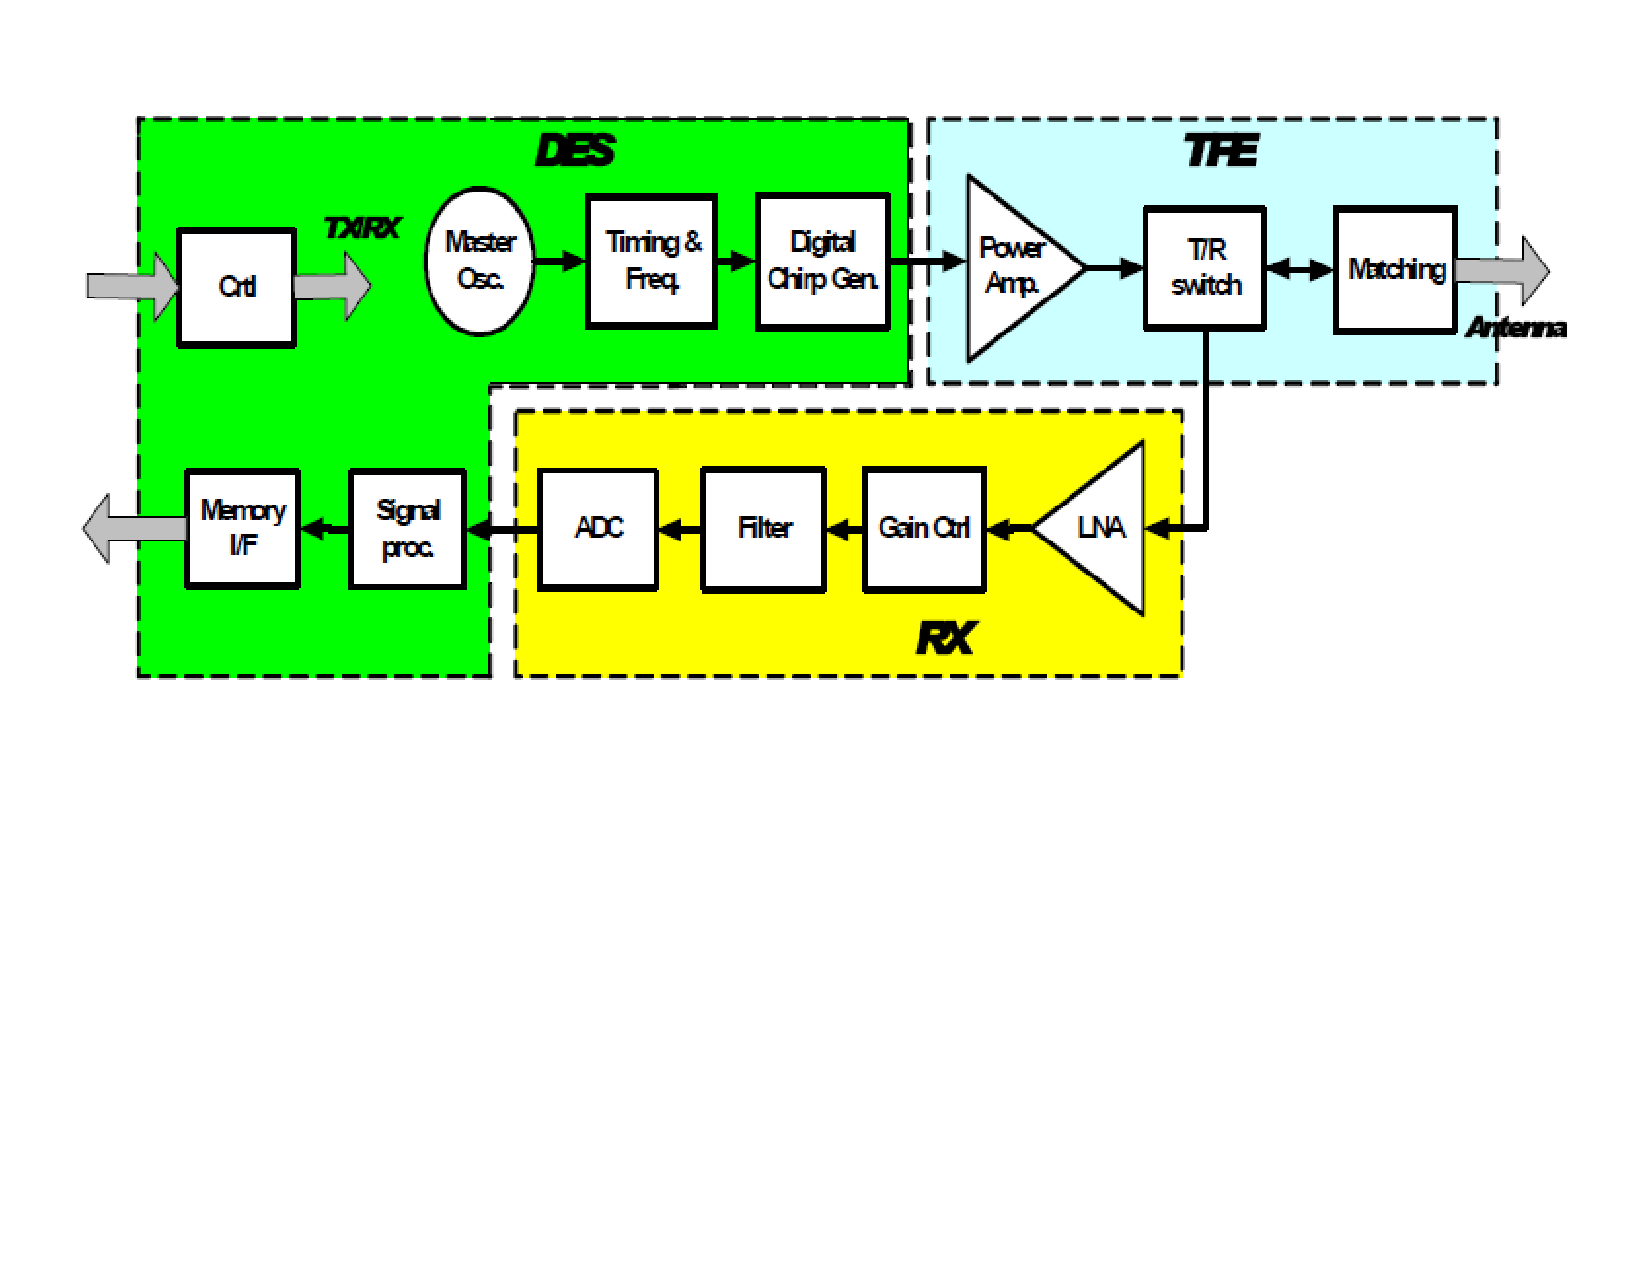
\includegraphics[scale=0.5]{Figures/IPR_Architecture.pdf}
\caption{Architecture of \ac{IPR} instrument \cite{IPR_performance}}
\label{fig:IPR_achitecture}
\end{figure}
%
\subsection{Instrument Characteristics}
The characteristics and parameters of the \ac{IPR} are listed in table \ref{tab:parameter} which are explained in the following subsections.\\

\begin{table}[H]
\centering
\caption{\ac{GIPER} instrument Parameters }
\label{tab:parameter}
\begin{tabular}{|c|c|}
\hline 	\textbf{Parameter}		&  \textbf{Value}\\ 
\hline  Orbit Altitude			&  $200$~km	\\ 
\hline  Centre Frequency		&  $45$~MHz		\\ 
\hline  Chirp Bandwidth			&  $10$~MHz		\\
\hline  PRF						&  $963.39$~Hz	\\  
\hline  Pulse Width				&  $85 \mathrm{~\mu s}$		\\ 
\hline  Ice Range Resolution	&  $8.6$~m		\\
\hline  Along Track Resolution	&  $817$~m		\\ 
\hline  Across Track Resolution	&  $4899$~m		\\ 
\hline  SNR						&  $14.7$~dB	\\ 
\hline  Power					&  $20$~W		\\ 
\hline  Mass					&  $10$~kg		\\ 
\hline 
\end{tabular} 
\end{table}
\subsubsection{Central Frequency and Bandwidth}
The radar frequency determines the penetration capability of the radar, while the bandwidth of the transmitted pulse determines range resolution \cite{penetrartion}. From the Jovian radiation spectrum as shown in figure \ref{fig:Jovian_radio_emission} measured at 1 AU, it is clear that the frequency cutoff for the Jovian radio emission affecting the subsurface radar is around 40 MHz. So, we choose 45 MHz as central frequency for the \ac{IPR} with 10 MHz bandwidth (40-50 MHz). This gives 3.6~m length for the dipole antenna. Assuming ice ($\epsilon_{r} = 3.2$), Vertical resolution of the \ac{IPR} is 8.4 m which is calculated from equation \ref{eq:range_resolution}.
%
\begin{equation}
\rho_{z} = \dfrac{c}{2B_{w}\sqrt{\epsilon_{r}}}
\label{eq:range_resolution}
\end{equation}
%
\begin{figure}[bht]
\centering
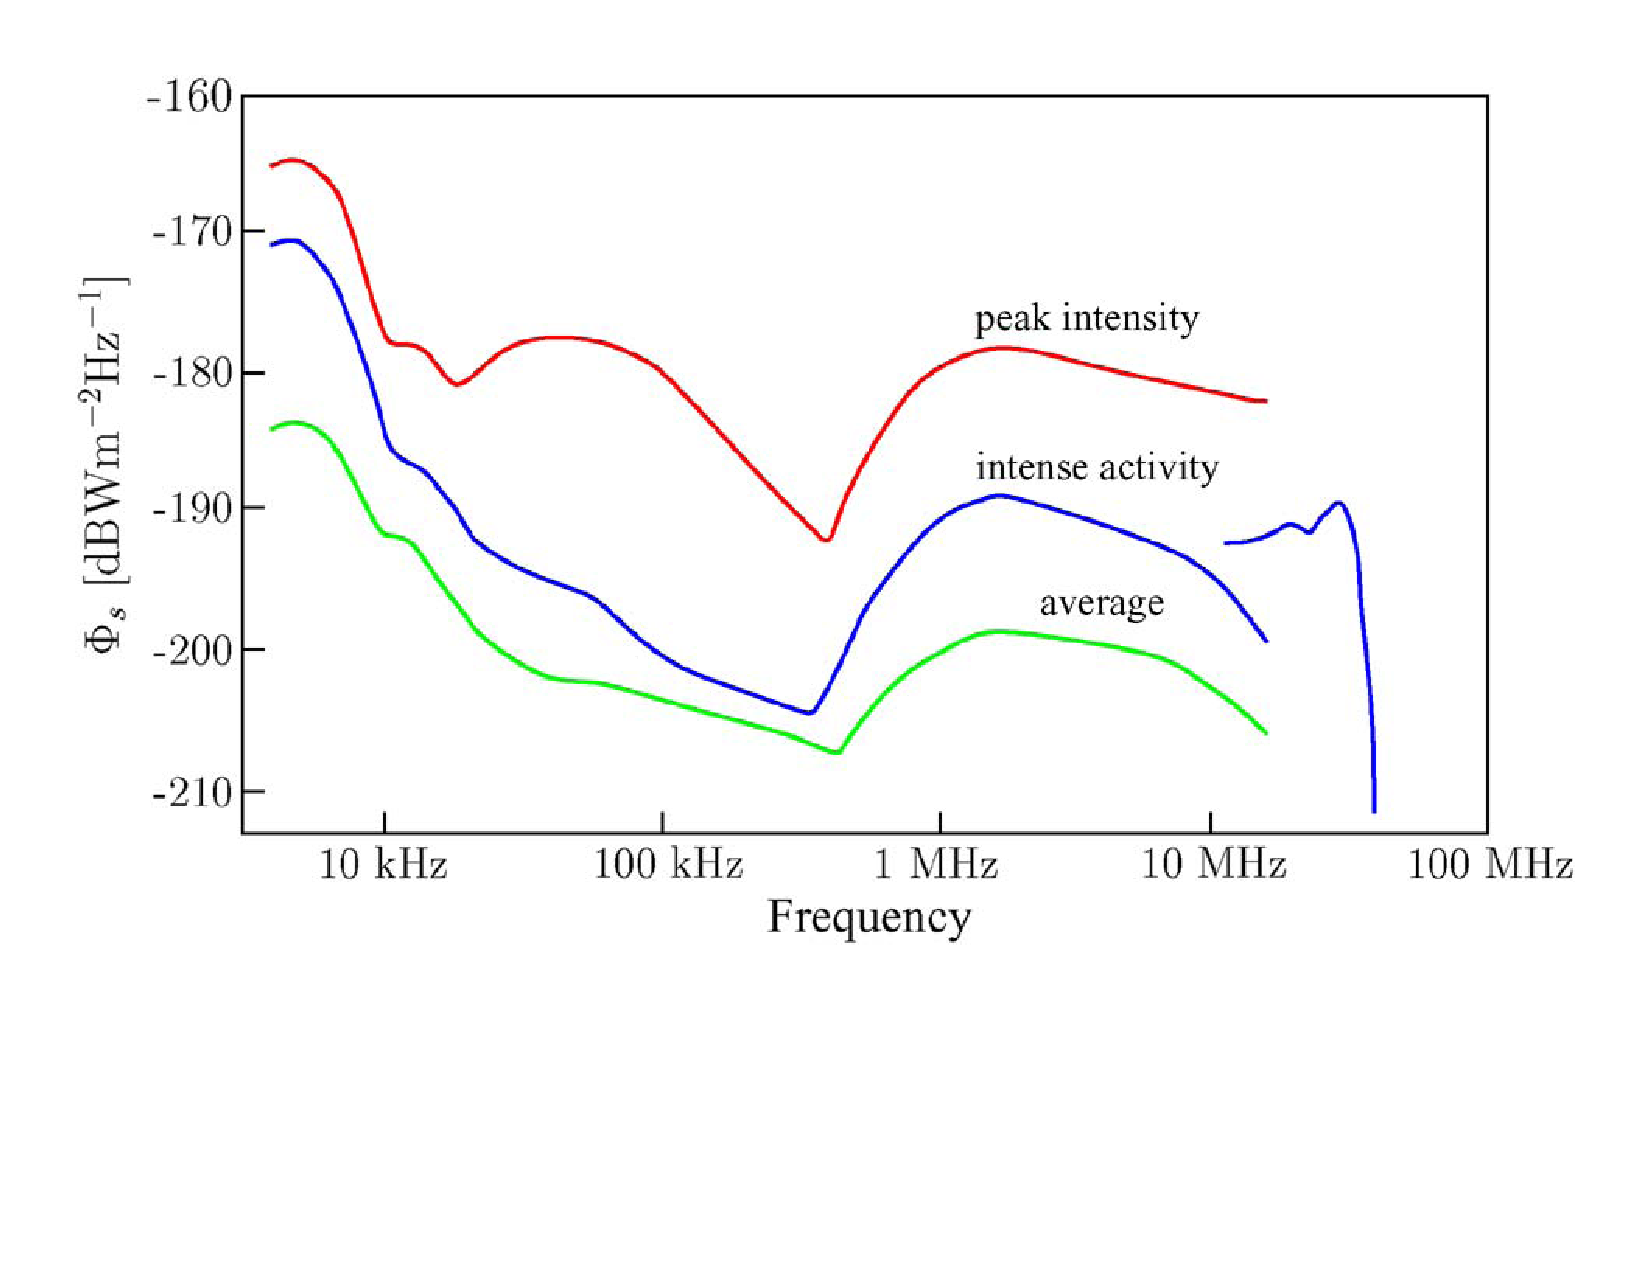
\includegraphics[scale=0.5]{Figures/Jovian_radio_emission.pdf}
\caption{Jovian radio emission spectrum \cite{Gany_SRS}} 
\label{fig:Jovian_radio_emission}
\end{figure}
%
\subsubsection{Pulse repetition frequency and pulse width}
The pulse width for the \ac{IPR} is $85 \mathrm{~\mu s} $ and \ac{PRI} is $1038 \mathrm{~\mu s}$; giving a duty cycle of $8.2\% $. This results in a \ac{PRF} of $963.39$~Hz. All these timings are shown in figure \ref{fig:PRI}. A receiving window of $165 \mathrm{~\mu s}$ is dedicated to receive the radar echoes. The size of the receiving window is calculated by adding a two way travel time in ice for $5$~km depth ($60 \mathrm{~\mu s}$), the chirp signal duration ($85\mathrm{~\mu s}$) and  a safety margin of $10 \mathrm{~\mu s}$ on each sides. The speed of the electromagnetic waves is reduced by a factor of $1.7$ in ice. A switching time of $177 \mathrm{~\mu s}$ from transmission to reception mode is incorporated as utilized in the \ac{SHARAD} design \cite{SHARAD}.
%
\begin{figure}[bht]
\centering
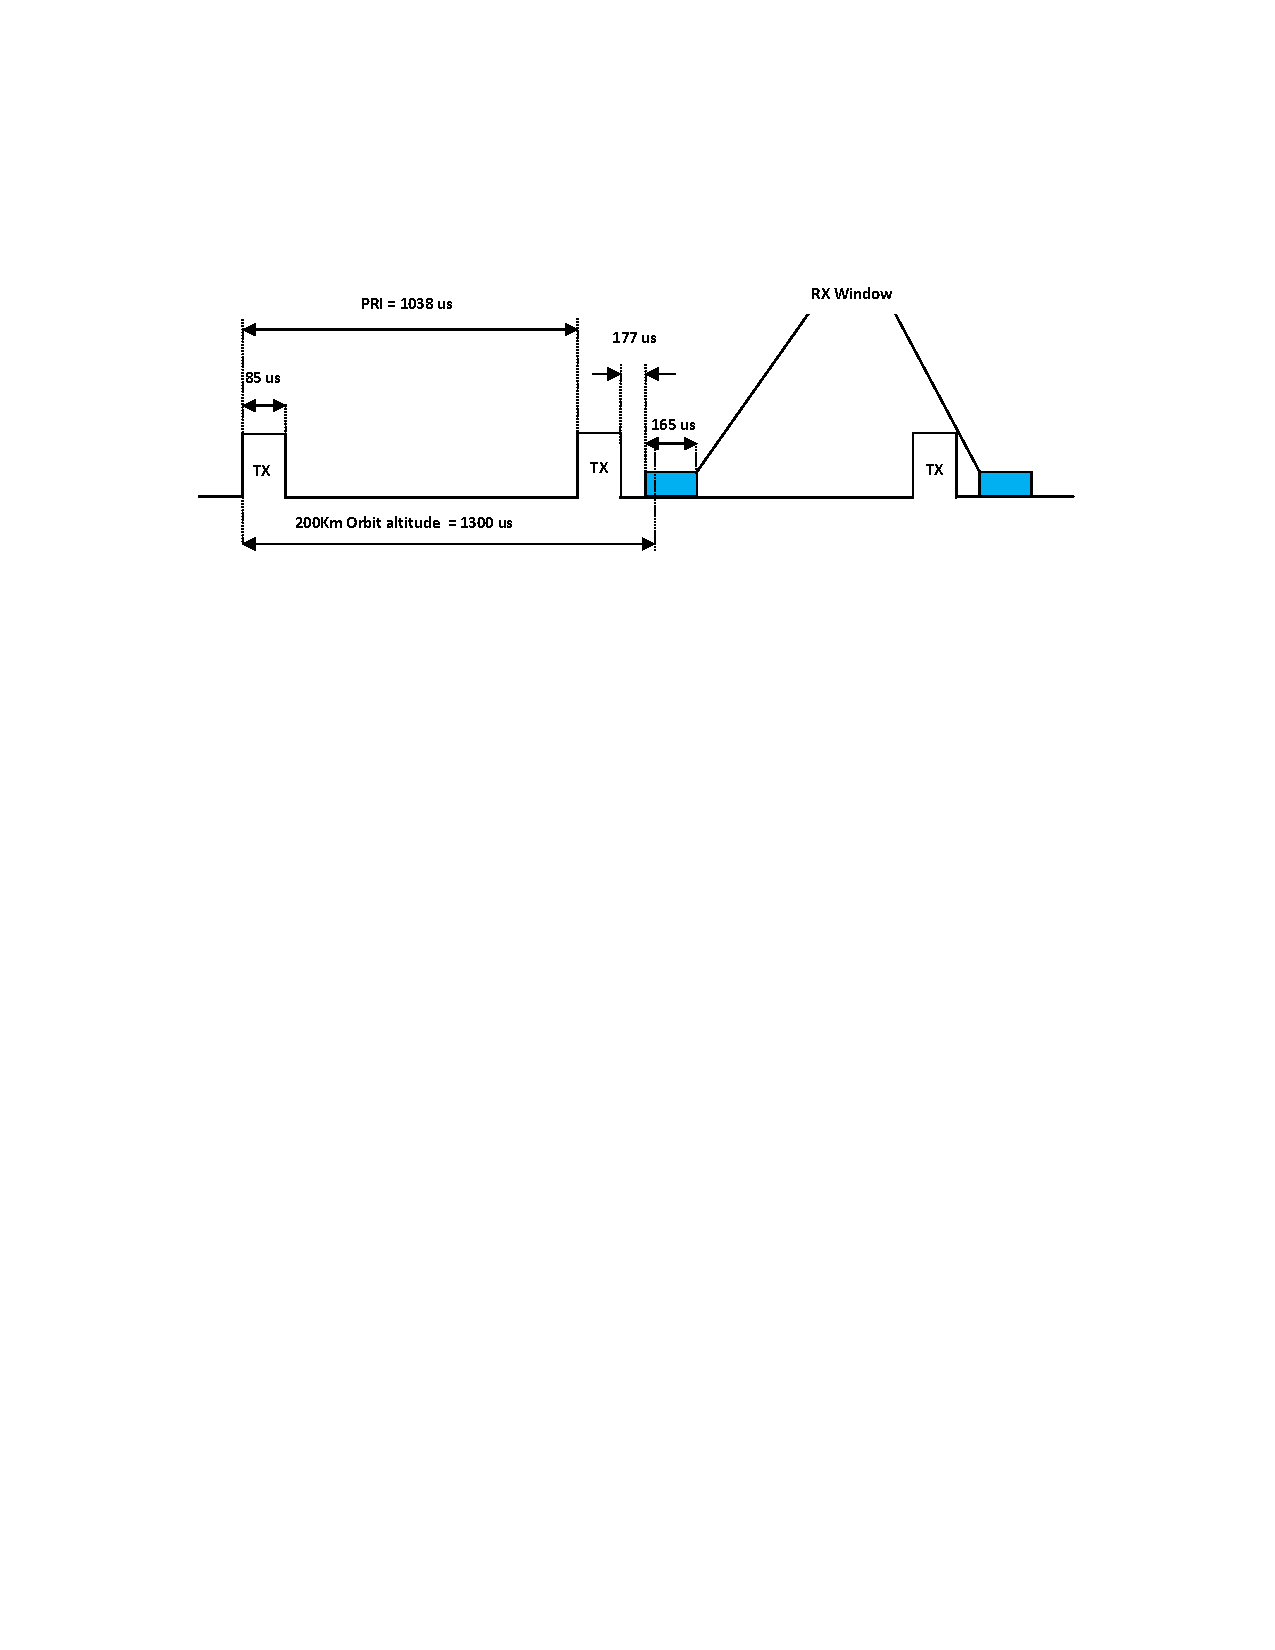
\includegraphics[scale=1]{Figures/PRI.pdf}
\caption{Timing diagram of Ganymede \ac{IPR}} 
\label{fig:PRI}
\end{figure}
%
\subsubsection{Ground Resolution}


The resolution of the system is determined by the nature of the target. Over specular surfaces (at the length scale of wavelength), where coherent reflection can be assumed, the resolution becomes that of the ``Fresnel circle'' which is 1633 m calculated using equation \ref{eq:fresenel_circle} from \cite{SHARAD}.
\begin{equation}
D_{f} = \sqrt{2h\lambda}
\label{eq:fresenel_circle}
\end{equation}
where $h$ is height and $D_{f}$ is Fresnel circle diameter.

Over rough surfaces, where incoherent scattering is assumed, the ground resolution is approximated with the first pulse limited resolution cell $D_{pl}$ as shown in figure \ref{fig:IPR_concept} . The first pulse-limited cell is represented by a circle on the ground centered in the nadir point, which diameter is given by the intersection of the wavefront with the ground surface when the transmitted wave has penetrated into the ground to a depth equal to $\rho_{z}$ \cite{Gany_SRS}. So worst case resolution for incoherent scattering calculated from equation \ref{eq:pulse_limited_cell} is 4899 m 
\begin{equation}
D_{pl} = 2\sqrt{\dfrac{hc}{B_{w}}}
\label{eq:pulse_limited_cell}
\end{equation}
However along track resolution can be improved using synthetic aperture processing which is explained in section \ref{SAR} using equation \ref{eq:along_track_resolution} which results in $817 m$. Effective integration time for unfocussed Doppler processing calculated by equation \ref{eq:integration_time} is $860 ms$ and the number of pulses used to make synthetic aperture is calculated by equation \ref{eq:Number_pulses} from \cite{Gany_SRS}  which comes out to 666 giving a processing gain of $28 dB$ 
%
\begin{equation}
L_{s} = \sqrt{\dfrac{h\lambda}{2}}
\label{eq:along_track_resolution}
\end{equation}
%
\begin{equation}
T_{i,eff} = \dfrac{D_{f}}{V_{s}}
\label{eq:integration_time}
\end{equation}
\begin{equation}
N = T_{i,eff}PRF 
\label{eq:Number_pulses}
\end{equation}
%
\subsubsection{Signal-to-Noise Ratio}

The power of the received echo is estimated from the classical radar equation. Using the \ac{IPR} design parameters from the table \ref{tab:parameter}, the expected power level of the surface echo is calculated. Here, two processing gains are exploited; one chirp processing gain of $29.3 dB$ given by equation \ref{eq:chirp gain} and second synthetic aperture processing gain of $28 dB$ given by equation \ref{eq:Number_pulses}. So after incorporating the processing gain, signal power from the Ganymede surface is given by equation \ref{eq:radar_basic} which is about $-91.7 dB$.

\begin{equation}
Pr_{s} = \dfrac{P_{t}\lambda^{2}G^{2}(\frac{D_{pl}}{2})^{2}\sigma_{o}}{(4\pi)^{3}h^{4}} 
	  = -91.7 dB 
\label{eq:radar_basic}
\end{equation}
where $P_{t}$ is the transmitted power, $Pr_{s}$ is the surface echo strength $\lambda$ is the wavelength  and $\sigma_{o}$ is the reflection coefficient of the target surface and is a statistical quantity which depends upon the dielectric properties of the two mediums at the interface and can be approximated by the Kirkhhoff model \cite{MIMOSA} and for space/ice interface it is equal to $-10 dB$ .
%
Then signal attenuation inside ice is estimated. Loss tangent from which the dielectric absorption is calculated depends upon the electromagnetic wave frequency and the temperature of the ice \cite{MIMOSA}. Assuming Ganymede surface temperature of 120 K and a slow linear increasing with depth of about 10 K within the first 5-km depth, \cite{Gany_SRS} calculated the attenuation of the radar signal for 20 MHz and 50 MHz. Interpolating the result for 45 MHz frequency, the attenuation is $1.2 dB per Km$ giving $12 dB$ loss for two way traversing of radar signal in 5 Km depth. So any echo after travelling $5 Km $ distance will be $103.7 dB$ plus the reflection coefficient of the subsurface layer which is given by equation \ref{eq:signal_strength}. The reflection coefficient estimated from the Kirkhhoff models for ice/rock and ice/water interface are $-11dB$ and $-3 dB$ respectively.
%
\begin{equation}
Pr_{ss} = -103.7 dB + 10 log \sigma_{oss}
\label{eq:signal_strength}
\end{equation}
where $Pr_{ss}$ is the subsurface echo and $\sigma_{oss}$ is the reflection coefficient of the subsurface layer.\\
Radar sensitivity is limited by the noise sources present in the measurement chain. These sources include Jovian emission, galactic noise and thermal noise of the receiver.  As the central frequency and the associated bandwidth of $10 MHz$ is away from the noisy Jovian spectrum so Jovian noise is not critical. Galactic noise temperature at $45 MHz$ is about $10^{5}K$ while the thermal temperature of the radar receiver will be about  $300 K$. As, the instrument temperature is quite low as compared to galactic noise so, we can ignore thermal noise of the receiver and the performance of the \ac{IPR} is only limited by the galactic noise which is calculated from equation \ref{eq:galactic_noise} and is equal to $-118.6 dB$. So signal to noise ($\frac{S}{N_{g}}$) ratio for surface echoe is about $26.9 dB$ while for the subsurface echo will be $14.9 dB$ plus reflection coefficient of the subsurface.
\begin{equation}
N_{g} = K_{B}T_{g}B_{w}
\label{eq:galactic_noise}
\end{equation}
\\


\subsubsection{Clutter Rejection and Synthetic Aperture Processing}
\label{SAR}
As the directivity of the dipole antenna is quite low which will illuminate a large surface area of the target. This will result in echoes coming from the off-nadir along with nadir direction as shown in figure \ref{fig:IPR_concept}. This off-nadir echoes called clutter can be divided into two parts; along the track clutter and across the track clutter.\\
%
Along the track clutter will be removed by the synthetic aperture processing technique which uses the relative motion between the spacecraft and target to synthesize a large aperture which is equal to the space covered during the integration time. As \ac{IPR} is a coherent radar, it measures and records the phase history of the received signals. In order to reduce on board computation and downlink data rate, Doppler processing is chosen unfocussed and moreover following the \ac{MARSIS} approach i.e., requiring that the signal phase variation during a synthetic aperture is smaller than $\pi/4$, the phase compensation of the echoes during the formation of a synthetic aperture is simpler and can be performed on board in real time, as only a linear phase compensation of the echoes is required \cite{Gany_SRS}. To ensure that only coherently resolved echoes from a contiguous Fresnel zone are being illuminated, the maximum along track integration distance is limited to the Fresnel zone given by equation \ref{eq:
fresenel_circle}.
\\
Across the track clutter is limited by the antenna pattern and will be removed by developing a simulator of the radar using a model of the overflown surface (accurately modelled at the scale of interest), which predicts the presence of clutter echoes. In this way, the corresponding echoes appearing in the measured radar-gram can be properly interpreted as clutter and then neglected \cite{SHARAD}. Some information for Ganymede was obtained through a \ac{DEM} produced from Voyager images. However, this is enough  for deriving \acp{DEM} of different portions of Ganymede for a better understanding of the clutter issue \cite{Gany_SRS}. As the instrument package of the \ac{JGO} mission includes radar altimeter so after modelling the Ganeymede surface, across the track clutter will be removed.
\subsection{Design feasibility}
The \ac{IPR} for the \ac{JGO} system is based on a mature and experienced technology that has flight heritage for two different Mars Missions (MARS Express, with the \ac{MARSIS} instrument; NASA Reconnaissance Orbiter with \ac{SHARAD} with slight variations to full fill  the mission objectives of the \ac{JGO}. From the link budget analysis, it is obvious that we have enough margin to detect the sub layer echoes.  Thus \ac{IPR} is capable of full filling the scientific objectives for the first $5 Km$ surface depth of Ganymede.
%
%thermal, power, mechanical mounting, EMC, especially radiation sensitive parts, radiation shielding and mitigation strategy, flight heritage of hardware, ressource budgets, 
%This mission assumes that an altimeter instrument is included in the JUICE mission scientific instrument package. Altimeter is needed to estimate the surface clutter and surface slope.
%
\section{Summary of Instrument Interfaces}
%data, mechanical, power, EMC, thermal,
An important requirement is to have always the antenna parallel to the ground during the measurements with accuracy of $\pm 5^{\deg}$. Concerning yaw, a deviation from parallel to the ground should be less than $1^{\deg}$. It is also important to have a small roll (<$ 10^{\deg}$) in order to have the maximum antenna beam pattern size at nadir \cite{yellowbook}.
%
\section{On-ground and In-flight Test and Calibration}
%test equipment requirements (i.e. thermal vacuum chamber, EMC labs etc.), EGSE, radar signal simulator(test of ground processing chain),
%
\begin{floatingfigure}[r]{0.3\textwidth}
\centering
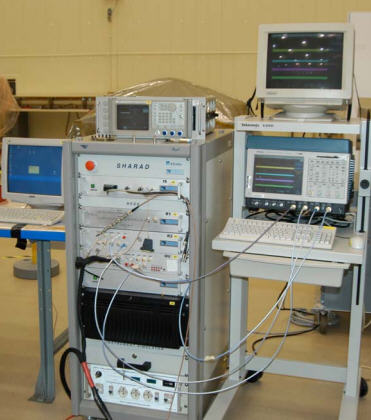
\includegraphics[width=0.27\textwidth]{Figures/MEGS}
\caption[caption]{Mars Echo Generation System used on the SHARAD instrument\cite{MEGS}}
\label{fig:MEGS}
\end{floatingfigure}
%
The \ac{GIPER} instrument will undergo a series of development and qualification tests to ensure that the instrument functions correctly and that it will achieve its scientific objectives. 
%
%
The required test facilities include \ac{EMC} lab, \ac{RF} lab, Thermal-Vacuum chamber, vibration and shock testing and a \ac{GIPER} raw signal simulator. Some test facilities are available within the \ac{GIPER} instrument group, some will be provided by the Swedish space industry and consortium partners. The instrument will require tests at ESA's \ac{RF} labs for testing of the \ac{GIPER} antenna radiation characteristics. A complete instrument test overview is shown in Table \ref{tab:instrument_testing}.
%
\vspace{15mm}
%
\subsection{EGSE}
A raw signal simulator will be developed by the \ac{GIPER} instrument group. This raw signal simulator will be similar to the one developed for the \ac{SHARAD} instrument\cite{Giovanni} as shown in figure \ref{fig:MEGS} and allow testing of the instrument signal processing chain and to develop a Ganymede transfer function considering the orbit altitude and surface clutter and sub-surface dielectric interfaces. After launch of the JUICE satellite, the \ac{GIPER} \ac{EGSE} will be located at the JUICE \ac{MOC}. A set of calibration files and algorithms will also be sent to the JUICE \ac{SOC} for processing of the raw instrument data into L1b data.
%
%
\subsection{In-Flight Calibration}
As was done for the SHARAD instrument\cite{SHARAD_ppt}, two types of in-flight calibrations are planned. An internal calibration is performed by directly looping a transmitted signal to the receiver and sending the raw unprocessed data to ground. An external calibration is performed by transmitting signals onto a flat surface region of Ganymede, receiving the echo and sending the unprocessed data to ground. These calibrations will be performed once the radar antenna has been successfully deployed.
%
%
\section{System Level Assembly, Integration and Verification}
%
Verification by testing will be the main method of verification for the \ac{GIPER} instrument. Other means of verification are analyses and mathematical models.  
%
\subsection{Requirements}
Of special concern to the \ac{GIPER} instrument performance and degradation is the intense radiation of high energy electrons which may affect the instrument electronics. Testing and verification must ensure that the instrument will meet is full operational performance when it enters its primary scientific operation phase at the spacecraft Ganymede orbit insertion ten years after launch.
%
\subsection{Deliverable Models}
%
The \ac{GIPER} instrument development will apply the following model philosophy:
%
\begin{itemize}
\item \ac{STM} - For testing of the instrument structural and thermal interface to the spacecraft\\
\item \ac{EM} - To test and verify that the instrument meets the functional and technical requirements.\\
\item \ac{PFM} - will be build using full flight standard components and tested at qualification levels and at acceptance durations. This will ensure that the specified instrument performance is met in accordance to the space environment found around Jupiter.
\end{itemize}
%
Before building of the \ac{PFM} is initiated, a dedicated \ac{QM} will be build and tested at qualification level. This unit can then later be refurbished as a \ac{FS} in case this deems necessary.
%%
\subsection{System Level Testing}
%
%
Table \ref{tab:instrument_testing} shown the test plan for each instrument model and the applied testing levels.
%
\begin{table}[H]
\centering
\caption{Instrument test levels for different instrument models (D=Development, Q=Qualification, P=Proto-flight)}
\label{tab:instrument_testing}
\begin{tabular}{p{0.40\textwidth}ccccp{0.25\textwidth}}
\hline
\textbf{Test} & \textbf{STM} & \textbf{EM} & \textbf{QM}& \textbf{PFM} & \textbf{Test Facilities}\\
\hline
Visual Inspections & - & - & - & P & LTU Rymdcampus\\
Mechanisms lifetime & Q & - & - & - & \ac{IRF}\\
Functional and Performance & - & D & Q & P & \ac{IRF}\\
Sine and Random Vibrations & Q & - & - & P & \ac{IRF}\\
Shock & Q & - & - & P &Chalmers University of Technology\cite{Jonsson}\\
Thermal Vacuum & - & D & Q & P & \ac{IRF}\\
EMC Conducted/Susceptibility & - & D & - & P &\\
RF Test & - & - & Q & - & ESA ESTEC\\
DC Magnetic Test & - & D & Q & P & \ac{IRF}\\
\hline
\end{tabular}
\end{table}
%
%
%
\section{Flight Operations Concept}
%operational modes, calibrations, 
%
The instrument modes are inherited from the SHARAD instrument\cite{SHARAD_ppt}.
%
\subsection{Nominal Operations}
%
Four nominal operation modes are defined:
\begin{itemize}
\item Low data rate
\item High data rate
\item Calibration
\item Receive only
\end{itemize}
%
\subsection{Other Modes}
%
Two silent modes are defined:
\begin{itemize}
\item Off - all equipments turned off
\item Heating - only heaters are powered on
\end{itemize}
%
Additionally, four support modes are defined: 
\begin{itemize}
\item Check/init
\item Standby
\item Warm-up
\item Idle
\end{itemize}
%
%
\section{Science Ground Segment Concept}
This section describes the preliminary expected GIPER contributions to the JUICE \ac{SGS}. These will later be further specified in the \ac{GIPER} \ac{SIP}.
%
\subsection{Implementation Concept for the Science Ground Segment}
A dedicated \ac{GIPER} \ac{SOG} will be established at LTU, Kiruna as has been done on previous instruments from \ac{IRF}\cite{ASPERA_PO}. %
%
\subsection{Planning of Payload Operations}
The \ac{GIPER} \ac{SOG} will provide the necessary support to the JUICE \ac{SOC} in preparation of the instrument science operations planning and scheduling.
%
\subsection{On-Board Software Maintenance}
During instrument commissioning and critical operation phases, the \ac{GIPER} \ac{SOG} may be relocated to the JUICE \ac{MOC} established at ESOC or \ac{SOC} at ESAC along with the \ac{EGSE}. 
%
%
\section{Data Reduction, Scientific Analysis and Archival Plans}
%
It is expected that housekeeping data and science data will be sent from the JUICE \ac{MOC}, via internet, to the \ac{GIPER} \ac{SOG} in LTU, Kiruna. Here data will be reduced, archived and distributed to other science teams including the JUICE science data archive. To correctly remove surface clutter signals, it is required to have simultaneously data from the altimeter instrument. 
%
A Quick-Look data analyser software will be developed, to optimise efficiency and scientific return of instrument operations.
%
A software tool will also be developed to analyse and convert L1b raw data values (un-calibrated science data) into L2/L3 data files.
%
\section{Organization}
%
The \ac{GIPER} instrument group is led by three SpaceMaster students from round 7. LTU and \ac{IRF} are supporting institutions.
%
\subsection{Management Structure}
%
\noindent
Jan Sommer is the instrument \ac{PI}. With a background in Physics and numerous courses and Space Science, he has a strong knowledge a Planetary Sciences and understanding of the underlying physics which will ensure that the \ac{GIPER} instrument will meet the scientific requirements.\\\\
%
\noindent
Morten Olsen is the project manager. With experience as project manager for previous space projects including CanSat and U-SPACE, he will manage the \ac{GIPER} project to ensure that deliverables are ready on schedule and within budget.\\\\
%
\noindent
Omair Sarwar is the technical manager. With a background in Aeronautical Engineering, experience with telecommunication systems and having studied radar courses, he will ensure that the \ac{GIPER} instrument meets the performance requirements, proper instrument verification and qualification in accordance with ESA space standards.
%
\subsection{Budget}
ACME Space Agency is the \ac{LFA} for this instrument proposal. A \ac{LOE} has been issued ensuring funding for the project during the instrument development phase, in-flight operations and post operations activities.